\section{Simulare F martie 2024}

2024.S.1. O baterie cu tensiunea electromotoare $E=12 \mathrm{~V}$ și rezistență internă neglijabilă, alimentează un circuit format din trei rezistoare: $R_{1}$ legat în serie cu gruparea formată din rezistoarele $R_{2}$, $R_{3}$ conectate în paralel. Cunoscând valorile rezistențelor $R_{1}=2 \Omega$, $R_{2}=6 \Omega$ şi intensitatea curentului prin circuit $I=2 \mathrm{~A}$, valoarea rezistenței $R_{3}$ este:\\ a) $12 \Omega$; b) $10 \Omega$; c) $5 \Omega$; d) $15 \Omega$; e) $14 \Omega$; f) $4 \Omega$.\\ Rezistența echivalentă a circuitului este:\\ $R_{e}=\frac{E}{I}=R_{1}+\frac{R_{2} R_{3}}{R_{2}+R_{3}}$.\\ De aici rezultă:\\ $R_{3}=\frac{\left(R_{e}-R_{1}\right) R_{2}}{R_{2}-R_{e}+R_{1}}=12 \Omega$. Răspuns corect a.\\

2024.S.2. Se consideră circuitul din figură, in care se neglijează rezistențele interne ale generatoarelor și se cunosc $E_{1}=2 \mathrm{~V}$, $E_{2}=5 \mathrm{~V}$ şi $R_{3}=2 \Omega$. Când curentul prin generatorul $\mathrm{E}_{1}$ este nul, cantitatea de căldură degajată prin rezistorul $R_{3}$ într-un interval de 2 ore, este:\\ a) $14,4 \mathrm{~kJ}$; b) $12,4 \mathrm{~kJ}$; c) $144 \mathrm{~J}$; d) $180 \mathrm{~J}$; e) $15 \mathrm{~J}$; f) $20 \mathrm{~J}$.\\ 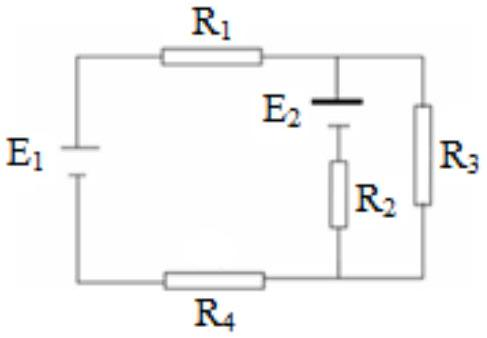
\includegraphics[width=0.4\linewidth]{images/2025_08_27_3bb07d46e3cd56c9410dg-1}\\ Folosim notațiile din figură:\\ \begin{center} 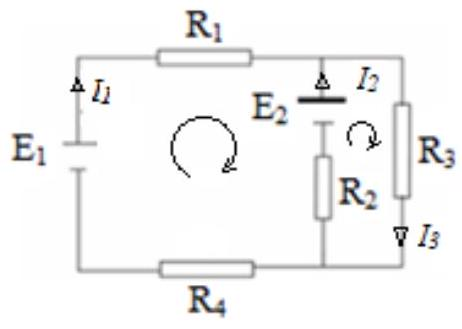
\includegraphics[width=0.4\linewidth]{images/2025_08_27_5ca5e43b13015248f3a3g-1} \end{center}\\ Aplicând legile lui Kirchhoff în cele două moduri de rețea și în cele două ochiuri de rețea ale circuitului obținem:\\ $I_{1}=I_{2}+I_{3}\\ E_{1}-E_{2}=I_{1} R_{1}-I_{2} R_{2}+I_{1} R_{4}\\ E_{2}=I_{3} R_{3}+I_{2} R_{2}$\\ Din condiția $I_{1}=0$ obţinem $I_{3}=-I_{2}$ și $E_{1}-E_{2}=I_{3} R_{2}$, de unde rezultă:\\ $R_{2}=\frac{E_{1}-E_{2}}{I_{3}}$ și $I_{3}=\frac{E_{1}}{R_{3}}$.\\ Energia disipată în rezistorul $R_{3}$ este:\\ $W=I_{3}^{2} \cdot R_{3} \cdot \tau=14400 \mathrm{~J}$. Răspuns corect a.\\

2024.S.3. De un tren cu masa $M=100 \mathrm{~t}$, care merge rectiliniu uniform, se desprinde ultimul vagon cu masa $m=10 \mathrm{~t}$. Puterea locomotivei este tot timpul constantă $P=300 \mathrm{~kW}$ iar după desprindere viteza trenului este tot constantă $v^{\prime}=72 \mathrm{~km} / \mathrm{h}$. Considerând că toate forțele de rezistență sunt direct proporționale cu greutatea, distanța parcursă de vagon până la oprire este:\\ a) $972 \mathrm{~m}$; b) $729 \mathrm{~m}$; c) $297 \mathrm{~m}$; d) $200 \mathrm{~m}$; e) $900 \mathrm{~m}$; f) $700 \mathrm{~m}$.\\ Înainte de desprinderea vagonului, viteza trenului este constantă, ceea ce înseamnă că forța de tracțiune $\left(F_{T}\right)$ este egală în modul cu forța de rezistență $\left(F_{R}\right)$. Cum forța de rezistență este proporțională cu greutatea trenului, rezultă:\\ $P=F_{T} \cdot v\\ F_{T}=F_{R}=\alpha \cdot M \cdot g$\\ De aici obținem viteza vagonului în momentul desprinderii: $v=\frac{P}{\alpha \cdot M \cdot g}$.\\ Vagonul se deplasează până la oprire sub acțiunea forței de rezistență\\ $F_{r}=\alpha \cdot m \cdot g$.\\ Din ecuaţia lui Galilei rezultă:\\ $v^{2}=\frac{2 F_{r}}{m} \cdot d$, de unde se obține $d=\frac{P^{2}}{2 \alpha^{3} \cdot g^{3} \cdot M^{2}}$.\\ După desprinderea vagonului, trenul se mişcă uniform cu viteza $v^{\prime}=72 \mathrm{~km} / \mathrm{h}$ având aceeași putere a motorului și forța de tracțiune $F_{T}^{\prime}=(M-m) g \cdot x$.\\ De aici rezultă $\alpha=\frac{P}{(M-m) g \cdot v^{\prime}}$ şi $d=\frac{v^{\prime 3}(M-m)^{3}}{2 P \cdot M^{2}}=972 \mathrm{~m}$. Răspuns corect a.\\

2024.S.4. În cursul unui proces în care volumul unui gaz ideal variază invers proporțional cu pătratul presiunii, se observă o creștere de două ori a presiunii. În acest caz, relația dintre temperatura finală și cea inițială este:\\ a) $T_{f}=T_{i} / 2$; b) $T_{f}=T_{i} \sqrt{2}$; c) $T_{f}=T_{i}$; d) $T_{f}=2 T_{i}$; e) $T_{f}=T_{i} / 4$; f) $T_{f}=4 T_{i}$.\\ Legea transformării descrise în problemă se scrie sub forma: $v \cdot P^{2}=c t$;\\ Din ecuația termică de stare rezultă:\\ $P_{i}^{2} v_{i}=\nu R T_{i} P_{i}\\ P_{f}^{2} v_{f}=\nu R T_{f} P_{f}$\\ De aici rezultă $T_{i} P_{i}=T_{f} P_{f}$, adică $T_{f}=\frac{T_{i}}{2}$. Răspuns corect a.\\

2024.S.5. Energia cinetică a unui corp este $E_{c}=10 \mathrm{~J}$. Lucrul mecanic efectuat asupra corpului pentru a-i dubla impulsul este:\\ a) $30 \mathrm{~J}$; b) $35 \mathrm{~J}$; c) $50 \mathrm{~J}$; d) $20 \mathrm{~J}$; e) $10 \mathrm{~J}$; f) $100 \mathrm{~J}$.\\ Din teorema de variație a energiei cinetice rezultă $\frac{m}{2}\left(v_{f}^{2}-v_{i}^{2}\right)=L$. Cum $p_{f}=2 p_{i}$ rezultă $v_{f}=2 v_{i}$, deci $L=\frac{m}{2} \cdot 3 v_{i}^{2}=3 E_{ci}=30 \mathrm{~J}$. Răspuns corect a.\\

2024.S.6. Căldura specifică la volum constant a unui gaz ideal cu masa molară $\mu=32 \mathrm{~g} / \mathrm{mol}$ și coeficientul adiabatic $\gamma=1,4$ este: (se cunoaște $\mathrm{R}=8,32 \mathrm{~J} / \mathrm{molK})$\\ a) $0,65 \mathrm{~J} / \mathrm{gK}$; b) $0,34 \mathrm{~J} / \mathrm{kgK}$; c) $0,63 \mathrm{~J} / \mathrm{gK}$; d) $0,3 \mathrm{~J} / \mathrm{kgK}$; e) $0,5 \mathrm{~J} / \mathrm{gK}$; f) $0,6 \mathrm{~J} / \mathrm{gK}$.\\ Din relația Robert-Mayer și definiția coeficientului adiabatic se obține:\\ $C_{v}=\frac{R}{(\gamma-1) \cdot \mu}=0,65 \frac{\mathrm{J}}{g \cdot \mathrm{K}}$. Răspuns corect a.\\

2024.S.7. Într-o mişcare uniform încetinită, viteza unui mobil la un moment dat este de $40 \mathrm{~m} / \mathrm{s}$, iar după $10 \mathrm{~s}$, corpul se oprește. Accelerația corpului este:\\ a) $4 \mathrm{~m} / \mathrm{s}^{2}$; b) $2 \mathrm{~m} / \mathrm{s}^{2}$; c) $1 \mathrm{~m} / \mathrm{s}^{2}$; d) $0,4 \mathrm{~m} / \mathrm{s}^{2}$; e) $0,2 \mathrm{~m} / \mathrm{s}^{2}$; f) $5 \mathrm{~m} / \mathrm{s}^{2}$.\\ Aplicând legea vitezei pentru mișcarea uniform variată obținem $a=\frac{v}{t}=4 \mathrm{~m} / \mathrm{s}$. Răspuns corect a.\\

2024.S.8. Două rezistoare cu rezistențele $R_{1}=2 \Omega$ și $R_{1}=4 \Omega$ se montează în serie apoi in paralel. Raportul rezistențelor echivalente este:\\ a) $4,5$; b) $4,2$; c) $5,2$; d) $9$; e) $2,5$; f) $5,4$.\\ Rezistența echivalentă a grupării serie este $R_{S}=R_{1}+R_{2}$ iar a grupării paralele este $R_{P}=\frac{R_{1} R_{2}}{R_{1}+R_{2}}$.\\ De aici raportul lor este: $\frac{R_{S}}{R_{P}}=\frac{\left(R_{1}+R_{2}\right)^{2}}{R_{1} R_{2}}=4,5$. Răspuns corect a.\\

2024.S.9. Lucrul mecanic efectuat de un gaz ideal într-o transformare izotermă în care volumul se dublează este:\\ a) $L=\nu R T \ln 2$; b) $L=R \ln \frac{1}{2}$; c) $L=\nu R \ln 2$; d) $L=\nu T \ln \frac{1}{2}$; e) $L=R T \ln \frac{1}{2}$; f) $L=R \ln 2$.\\ Lucrul mecanic într-o transformare izotermă este: $L=\nu R T \ln \frac{V_{f}}{V_{i}}$. Pentru situația dată, $V_{f}=2 V_{i}$. Răspuns corect a.\\

2024.S.10. Un corp punctiform alunecă fără frecare pe suprafața unui cilindru cu raza $R=5 \mathrm{~m}$ de-a lungul arcului de cerc $PO$. Accelerația gravitațională este $g=10 \mathrm{~m} / \mathrm{s}^{2}$. Dacă viteza inițială a corpului este egală cu $0 \mathrm{~m} / \mathrm{s}$, viteza în punctul $O$ este:\\ a) $10 \mathrm{~m} / \mathrm{s}$; b) $20 \mathrm{~m} / \mathrm{s}$; c) $5 \mathrm{~m} / \mathrm{s}$; d) $2 \mathrm{~m} / \mathrm{s}$; e) $12 \mathrm{~m} / \mathrm{s}$; f) $15 \mathrm{~m} / \mathrm{s}$.\\ 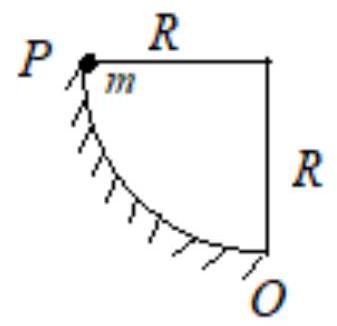
\includegraphics[width=0.4\linewidth]{images/2025_08_27_3bb07d46e3cd56c9410dg-2}\\ Din legea conservării energiei mecanice rezultă:\\ $\frac{m v^{2}}{2}=m g R \Righarrow v=\sqrt{2 g R}=10 \mathrm{~m} / \mathrm{s}$. Răspuns corect a.\\

